\chapter{Photon Interaction Physics and Sampling Derivations}
\label{ch:appendix_B}
In chapter \ref{ch:photon_interactions} the derivation of several important
equations were omitted. In this appendix the details of several derivations will
be shown in detail. In particular, the derivation of the outgoing energy of a
photon after a Compton scatter off of a free electron, the electron momentum 
projection on the photon scattering vector from a Compton scatter off of a
bound electron, the Klein-Nishina cross section differential in the inverse
energy loss ratio (x), the total Klein-Nishina cross section, Kahn's
rejection sampling technique, and the pair and triplet production thresholds
will be discussed.

\section{Compton Scattering from Free and Bound Electrons}
The process of Compton scattering off of a free electron is represented by 
figure \ref{fig:compton_scatter_free_electron}. Conservation of energy and 
momentum will be used to determine the final energy of the photon after the 
collision with the electron. First, the momentum of the particle system will be 
analyzed. In the transverse direction, momentum conservation is as follows.
\begin{equation*}
  P\sin{\theta} = P_e\sin{\phi}
\end{equation*}
In the longitudinal direction, momentum conservation is as follows.
\begin{equation*}
  P^{'} = P\cos{\theta} + P_e\cos{\phi} 
\end{equation*}
Both of these equations will now be squared and added together.
\begin{align}
  P^{'2} - 2P^{'}P\cos{\theta} + P^2(cos^2\theta + sin^2\theta) & = 
  P_e^2(cos^2\phi + sin^2\phi) \nonumber \\
  P_e^2 = P^{'2} - 2P^{'}P\cos{\theta} + P^2
\end{align}
This equation for the electron momentum will be useful in the equation for
the conservation of energy of the particle system.

Now, the energy of the particle system will be analyzed. The energy of the
system is shown below.
\begin{equation*}
  E^{'} + m_ec^2 = E + E_e
\end{equation*}
\begin{equation*}
  E^{'}-E + m_ec^2 = E_e
\end{equation*}
\begin{equation*}
  (P^{'} - P)c + m_ec^2 = \sqrt{\left(P_ec\right)^2 + \left(m_ec^2\right)^2}
\end{equation*}
\begin{equation*}
  (P^{'} - P)^2c^2 + 2m_ec^3(P^{'} - P) + m_e^2c^4 = P_e^2c^2 + m_e^2c^4
\end{equation*}
\begin{equation*}
  P^{'2}c^2 - 2P^{'}Pc^2 + P^2c^2 + 2m_ec^3(P^{'} - P) = P^{'2}c^2 - 
  2P^{'}P\cos{\theta}c^2 + P^2c^2
\end{equation*}
\begin{equation*}
  2m_ec^3(P^{'} - P) = 2P^{'}Pc^2(1 - \cos{\theta})
\end{equation*}
\begin{equation*}
  m_ec^3P^{'} = Pc(P^{'}c(1 - \cos{\theta}) + m_ec^2)
\end{equation*}
\begin{align}
  E & = \frac{m_ec^2E^{'}}{E^{'}(1 - \cos{\theta}) + m_ec^2} \nonumber \\
  & = \frac{E^{'}}{1 + \frac{E^{'}}{m_ec^2}(1 - \cos{\theta})} \\
  \alpha & = \frac{\alpha^{'}}{1 + \alpha^{'}(1 - \cos{\theta})} 
\end{align}

\begin{figure}[t!]
  \begin{center}
    \scalebox{1.0}{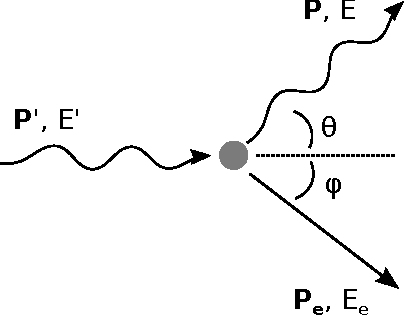
\includegraphics{backmatter/appendix_B/compton_scatter_free_electron.pdf}}
  \end{center}
  \caption{\textbf{Compton scattering off of a free electron.}}
  \label{fig:compton_scatter_free_electron}
\end{figure}

The process of Compton scattering off of a bound electron is represented by
figure \ref{fig:compton_scatter_bound_electron}.
\begin{figure}[t!]
  \begin{center}
    \scalebox{1.0}{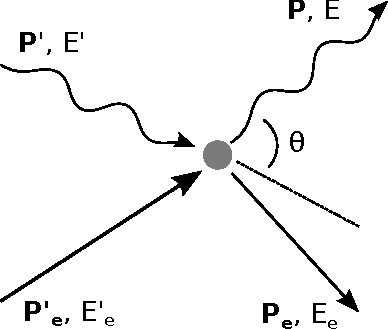
\includegraphics{backmatter/appendix_B/compton_scatter_bound_electron.pdf}}
  \end{center}
  \caption{\textbf{Compton scattering off of a bound electron.}}
  \label{fig:compton_scatter_bound_electron}
\end{figure}
Conservation of energy and momentum will again be used to determine the 
quantity of interest, which in this case is the initial electron momentum, 
$\vec{P_e^{'}}$, projected onto the photon scattering vector, 
$\vec{P} - \vec{P^{'}}$. The z-axis of the system will be set parallel to the
scattering vector. Therefore, the electron momentum projection will be 
represented by the variable $p_z$.

Before analyzing the energy of the particle system, then energy of the 
electron will be discussed. The kinetic energy of the electron will be
represented by, $E_{e,k}$.
\begin{align}
  E_e^2 & = m_e^2c^4 + P_e^2c^2 \nonumber \\
  & = \left(m_ec^2 + E_{e,k}\right)^2 \nonumber
\end{align}
\begin{equation}
  P_e^2c^2 = 2m_ec^2E_{e,k} + E_{e,k}^2
\end{equation}
The energy of the particle system is given below. The binding energy of the 
electron is $E_b$.
\begin{equation*}
  E^{'} + E_{e,k}^{'} + m_ec^2 = E + E_{e,k} + m_ec^2 + E_b
\end{equation*}
\begin{align}
  E^{'}-E-E_b & = E_{e,k} - E_{e,k}^{'} \nonumber \\
  \left(E^{'}-E-E_b\right)^2 & = \left(E_{e,k} - E_{e,k}^{'}\right)^2 \nonumber \\
  & = E_{e,k}^2 - 2E_{e,k}E_{e,k}^{'} + E_{e,k}^{'2} \nonumber \\
  & = P_e^2c^2 - 2m_ec^2E_{e,k} - 2E_{e,k}E_{e,k}^{'} + P_e^{'2}c^2 - 2m_ec^2E_{e,k}^{'}
  \nonumber \\
  & = \left(P_e^2 + P_e^{'2}\right)c^2 - 2m_ec^2E_{e,k}^{'} - 
  2E_{e,k}\left(m_ec^2 + E_{e,k}^{'}\right) \nonumber \\
  & = \left(P_e^2 + P_e^{'2}\right)c^2 - 2m_ec^2E_{e,k}^{'} - 
  2\left(E^{'}-E-E_b+E_{e,k}^{'}\right)\left(m_ec^2 + E_{e,k}^{'}\right) \nonumber\\
  & = \left(P_e^2 + P_e^{'2}\right)c^2 - 4m_ec^2E_{e,k}^{'} - 2E_{e,k}^{'2} -
  2\left(E^{'}-E-E_b\right)\left(m_ec^2 + E_{e,k}^{'}\right) \nonumber \\
  & = \left(P_e^2 - P_e^{'2}\right)c^2 -
  2\left(E^{'}-E-E_b\right)\left(m_ec^2 + E_{e,k}^{'}\right) \nonumber \\
  \left(P_e^2 - P_e^{'2}\right)c^2 & = \left(E^{'}-E-E_b\right)^2 +
  2\left(E^{'}-E-E_b\right)\left(m_ec^2 + E_{e,k}^{'}\right)
\end{align}

The momentum of the particle system will now be analyzed. 
\begin{align}
  \vec{P^{'}} + \vec{P_e^{'}} & = \vec{P} + \vec{P_e} \nonumber \\
  m_ec\vec{\alpha^{'}} + \vec{P_e^{'}} & = m_ec\vec{\alpha} + \vec{P_e} \nonumber
\end{align}
The new variable $\vec{\alpha}$ is simply the momentum of the photon in 
units of $m_ec$. The magnitude of this vector has the following properties.
\begin{align}
  \left|\vec{\alpha}\right| & = \alpha \nonumber \\
  & = \frac{P}{m_ec} \\ 
  & = \frac{E}{m_ec^2} 
\end{align}
The equation for the momentum of the system must be rearranged further before
moving on.
\begin{align}
  \vec{P_e^{'}} - \vec{P_e} & = \vec{q} \nonumber \\
  & = m_ec\left(\vec{\alpha} - \vec{\alpha^{'}}\right) \nonumber
\end{align}
\begin{align}
  q^2 & = (m_ec)^2\left|\vec{\alpha} - \vec{\alpha^{'}}\right| \nonumber \\
  & = (m_ec)^2\left(\alpha^{'2} + \alpha^2 - 
  2\vec{\alpha^{'}}\cdot\vec{\alpha}\right) \nonumber \\
  & = (m_ec)^2\left(\alpha^{'2} + \alpha^2 - 2\alpha^{'}\alpha\cos{\theta}\right)
\end{align}

Now, using the equation for $\vec{q}$, the equation for the electron momentum 
projection can be determined.
\begin{equation*}
  \vec{P_e} = \vec{P_e^{'}} - \vec{q}
\end{equation*}
\begin{equation*}
  P_e^2 = P_e^{'2} + q^2 - 2\vec{P_e^{'}}\cdot\vec{q}
\end{equation*}
\begin{equation*}
  2\vec{P_e^{'}}\cdot\vec{q} = -\left(P_e^2 - P_e^{'2}\right) + q^2
\end{equation*}
\begin{equation*}
  2p_zq = -\left(P_e^2 - P_e^{'2}\right) + q^2 \nonumber
\end{equation*}
\begin{align}
  p_z & = \frac{1}{2q}\left[-\left(P_e^2 - P_e^{'2}\right) + q^2\right] 
  \nonumber \\
  & = \frac{1}{2qc^2}\left[-(E^{'}-E-E_b)^2 - 2(E^{'}-E-E_b)(m_ec^2+E_{e,k}^{'})
    +q^2c^2\right] \nonumber \\
  & = \frac{m_e^2c^4}{2qc^2}\left[
    -\left(\alpha^{'}-\alpha-\frac{E_b}{m_ec^2}\right)^2 -
    2\left(\alpha^{'}-\alpha-\frac{E_b}{m_ec^2}\right)
    \left(1 + \frac{E_{e,k}^{'}}{m_ec^2}\right) + 
    \left|\vec{\alpha} - \vec{\alpha^{'}}\right|^2\right] \nonumber \\
  & = \frac{m_e^2c^2}{2q}\Bigg[-(\alpha^{'}-\alpha)^2 + 
    2(\alpha^{'}-\alpha)\left(\frac{E_b}{m_ec^2}\right) - 
    \left(\frac{E_b}{m_ec^2}\right)^2 -
    2(\alpha^{'}-\alpha)\left(1 + \frac{E_{e,k}^{'}}{m_ec^2}\right) + \nonumber \\
  & \qquad \qquad \qquad
    2\left(\frac{E_b}{m_ec^2}\right)\left(1 + \frac{E_{e,k}^{'}}{m_ec^2}\right) +
    \alpha^{'2} + \alpha^2 - 2\alpha^{'}\alpha\cos{\theta}\Bigg] \nonumber \\
  & = m_ec\frac{\left[(\alpha^{'}-\alpha)\left(1 + \frac{E_{e,k}^{'} - E_b}{m_ec^2}
    \right) + \alpha^{'}\alpha(1-\cos{\theta}) -
    \frac{1}{2}\left(\frac{E_b}{m_ec^2}\right)^2 + 
    \left(\frac{E_b}{m_ec^2}\right)\left(1 + \frac{E_{e,k}^{'}}{m_ec^2}\right)
    \right]} {\sqrt{\alpha^{'2} + \alpha^2 - 2\alpha^{'}\alpha\cos{\theta}}}
\end{align}
If the binding energy and kinetic energy of the electron are assumed to be 
small compared to the rest mass energy of the electron, they can be neglected. 
The resulting equation, which is often reported in the literature is the 
following.
\begin{equation}
  p_z = m_ec\frac{\left[\alpha - \alpha^{'} + \alpha^{'}\alpha(1-\cos{\theta})
      \right]}{\sqrt{\alpha^{'2} + \alpha^2 - 2\alpha^{'}\alpha\cos{\theta}}}
\end{equation}

Derivations that are similar to the ones just shown were completed by Sood
\citep{sood_doppler_2004}. 

\section{The Klein-Nishin Cross Section Differential in Inverse Energy Loss Ratio}
As mentioned in chapter \ref{ch:photon_interactions}, the differential 
Klein-Nishina cross section is most easily sampled when a change of variables
from steradians to the inverse energy loss ratio is conducted. The energy loss
ratio, which was originally shown in chapter \ref{ch:photon_interactions}, will
be shown again below.
\begin{align}
  \frac{1}{x} & = \frac{\alpha}{\alpha^{'}} \nonumber \\
  & = \frac{1}{1+\alpha^{'}(1-\cos{\theta})} \nonumber
\end{align}

The change of variables is conducted using the following relationship.
\begin{equation*}
  \frac{d\sigma_{K.N.}(x)}{dx} dx = 
  \frac{d\sigma_{K.N.}(\alpha^{'},\theta)}{d\Omega} d\Omega
\end{equation*}
\begin{equation*}
  \frac{d\sigma_{K.N.}(x)}{dx} = 
  \frac{d\sigma_{K.N.}(\alpha^{'},\theta)}{d\Omega}
  \left(\frac{d\Omega}{dx}\right)
\end{equation*}
Based on the equation for the energy loss ratio, the second term in the above
equation can be determined.
\begin{align}
  x = 1 + \alpha^{'}(1-\cos{\theta}) \nonumber \\
  dx = -\alpha^{'} d(\cos{\theta}) \nonumber
\end{align}
\begin{align}
  \frac{d\Omega}{dx} & = -2\pi\frac{d(\cos{\theta})}{dx} \nonumber \\
  & = \frac{2\pi}{\alpha^{'}}
\end{align}
The following relationships will also be useful while conducting the change
of variables.
\begin{align}
  x - 1 & = \alpha^{'}(1-\cos{\theta}) \\
  \cos{\theta} & = 1 - \frac{x - 1}{\alpha^{'}} \nonumber \\
  cos^2\theta & = 1 - \frac{2(x-1)}{\alpha^{'}} + \frac{(x-1)^2}{\alpha^{'2}}
\end{align}
Now, the change of variables can be completed.
\begin{align}
  \frac{d\sigma_{K.N.}(x)}{dx} & = \frac{r_e^2}{2}
  \frac{\left[1 + \cos{^{2}\theta} + \frac{\alpha^{'2}(1-\cos{\theta})^2}
                                  {1 + \alpha^{'}(1-\cos{\theta})}\right] }
  {\left[1 + \alpha^{'}(1-\cos{\theta}) \right]^2} 
  \left(\frac{2\pi}{\alpha^{'}}\right) \nonumber \\
  & = \left(\frac{\pi r_e^2}{\alpha^{'}x^2}\right)
  \left[1 + 
    \left(1 - \frac{2(x-1)}{\alpha^{'}} + \frac{(x-1)^2}{\alpha^{'2}}\right) +
    \frac{(x-1)^2}{x} \right] \nonumber \\
  & = \left(\frac{\pi r_e^2}{\alpha^{'}x^2}\right) \left[2 - 
    \frac{2x}{\alpha^{'}} - \frac{2}{\alpha^{'}} +\frac{x^2}{\alpha^{'2}} -
    \frac{2x}{\alpha^{'2}} + \frac{1}{\alpha^{'2}} + x - 2 + \frac{1}{x} \right]
  \nonumber \\
  & = \left(\frac{\pi r_e^2}{\alpha^{'}}\right) \left[ \frac{1}{\alpha^{'2}} +
    \frac{1}{x}\left(1 - \frac{2}{\alpha^{'}}-\frac{2}{\alpha^{'2}}\right) +
    \frac{1}{x^2}\left(\frac{2}{\alpha^{'}} + \frac{1}{\alpha^{'2}}\right) +
    \frac{1}{x^3} \right] \nonumber \\
  & = K \left[A + \frac{B}{x} + \frac{C}{x^2} + \frac{D}{x^3}\right]
\end{align}
\begin{align}
  K & = \frac{\pi r_e^2}{\alpha^{'}} \nonumber \\
  A & = \frac{1}{\alpha^{'}} \nonumber \\
  B & = 1 - \frac{2(\alpha^{'}+1)}{\alpha^{'2}} \nonumber \\
  C & = \frac{(1+2\alpha^{'})}{\alpha^{'2}} \nonumber \\
  D & = 1 \nonumber 
\end{align}

\section{The Total Klein-Nishina Cross Section}
Using the sampling methods from chapter \ref{ch:photon_interactions} will 
sometimes require the total Klein-Nishina cross section. Using the 
Klein-Nishina cross section differential in the inverse energy loss ratio,
the total Klein-Nishina cross section can be determined rather easily. The
integration of the differential cross section will be split up into four parts
and then recombined and reorganized to give the total cross section reported by 
Lux (with the error corrected) \citep{lux_monte_1991}. 
\begin{align}
  \sigma_{K.N.}(\alpha^{'}) & = \int_1^{1+2\alpha^{'}} \frac{d\sigma_{K.N.}(x)}{dx} dx
  \nonumber \\
  & = K \left(\int_1^{1+2\alpha^{'}} A dx + 
    \int_1^{1+2\alpha^{'}} \frac{B}{x} dx + 
    \int_1^{1+2\alpha^{'}} \frac{C}{x^2} dx + 
    \int_1^{1+2\alpha^{'}} \frac{D}{x^3} dx \right) \nonumber \\
  & = K \left(Ax \Bigg|_1^{1+2\alpha^{'}} + B\ln{x}\Bigg|_1^{1+2\alpha^{'}} -
    \frac{C}{x} \Bigg|_1^{1+2\alpha^{'}} - \frac{D}{2x^2} \Bigg|_1^{1+2\alpha^{'}}
    \right) \nonumber \\
  & = K \left(2\alpha^{'}A + B\ln{(1+2\alpha^{'})} - \frac{C}{1+2\alpha^{'}} + C -
    \frac{D}{2(1+2\alpha^{'})^2} + \frac{D}{2} \right) \nonumber \\
  & = K \left(\frac{2}{\alpha^{'}} + \ln{(1 + 2\alpha^{'})} -
    \frac{2(\alpha^{'}+1)}{\alpha^{'2}}\ln{(1+2\alpha^{'})} - 
    \frac{1}{\alpha^{'2}} + \frac{1+2\alpha^{'}}{\alpha^{'2}} - 
    \frac{1}{2(1+2\alpha^{'2})^2} + \frac{1}{2} \right) \nonumber \\
  & = K \left(\frac{2}{\alpha^{'}} + \ln{(1 + 2\alpha^{'})} -
    \frac{2(\alpha^{'}+1)}{\alpha^{'2}}\ln{(1+2\alpha^{'})} + 
    \frac{2}{\alpha^{'}} + \frac{2\alpha^{'}(1+\alpha^{'})}{(1+2\alpha^{'})^2} 
    \right) \nonumber \\
  & = K \left(\frac{4(1+\alpha^{'})^2}{\alpha^{'}(1+2\alpha^{'})} - 
      \frac{4\alpha^{'}}{1+2\alpha^{'}} + \ln{(1 + 2\alpha^{'})} -
    \frac{2(\alpha^{'}+1)}{\alpha^{'2}}\ln{(1+2\alpha^{'})} + 
    \frac{2\alpha^{'}(1+\alpha^{'})}{(1+2\alpha^{'})^2} 
    \right) \nonumber \\
  & = K \left(\frac{2(1+\alpha^{'})}{\alpha^{'}} 
    \left[\frac{2(1+\alpha^{'})}{1+2\alpha^{'}} - 
    \frac{\ln{(1+2\alpha^{'})}}{\alpha^{'}} \right] + \ln{(1 + 2\alpha^{'})} -
    \frac{4\alpha^{'}}{1+2\alpha^{'}} + 
    \frac{2\alpha^{'}(1+\alpha^{'})}{(1+2\alpha^{'})^2} \right) \nonumber \\
  & = K \left(\frac{2(1+\alpha^{'})}{\alpha^{'}} 
    \left[\frac{2(1+\alpha^{'})}{1+2\alpha^{'}} - 
    \frac{\ln{(1+2\alpha^{'})}}{\alpha^{'}} \right] + \ln{(1 + 2\alpha^{'})} -
    \frac{2\alpha^{'}(1+3\alpha^{'})}{(1+2\alpha^{'})^2} \right) \nonumber \\
  & = 2\pi r_e^2 \left(\frac{(1+\alpha^{'})}{\alpha^{'2}} 
    \left[\frac{2(1+\alpha^{'})}{1+2\alpha^{'}} - 
    \frac{\ln{(1+2\alpha^{'})}}{\alpha^{'}} \right] +
    \frac{\ln{(1 + 2\alpha^{'})}}{2\alpha^{'}} - 
    \frac{(1+3\alpha^{'})}{(1+2\alpha^{'})^2} \right) 
\end{align}

In the equation for the total Klein-Nishina cross section reported by Lux, the
second and third terms have an error \citep{lux_monte_1991}. The second term is
\begin{equation*}
  \frac{\ln{(1 + 2\alpha^{'})}}{2\alpha^{'}}.
\end{equation*}
In the equation reported by Lux, this term is
\begin{equation*}
  \frac{\ln{(1 + 2\alpha^{'})}}{2\alpha^{'2}}.
\end{equation*}
The third term is 
\begin{equation*}
  -\frac{(1+3\alpha^{'})}{(1+2\alpha^{'})^2}.
\end{equation*}
In the equation reported by Lux, this term is
\begin{equation*}
  -\frac{(1+3\alpha^{'})}{\alpha^{'}(1+2\alpha^{'})^2}.
\end{equation*}
